With the \pp-collision datasets collected during Run~2 of the LHC,
direct searches for non-resonant Higgs boson pair production
constitute the most sensitive probes of the Higgs boson self-coupling
constant, \lambdahhh. This is due to the large sensitivity of the
% total and differential
non-resonant \HH production cross section to anomalous values of
\lambdahhh. Hereafter, the self-coupling constant is given in terms of
the modifier $\klambda = \lambdahhh / \lambdahhh^{\text{SM}}$ relating
an assumed value of the self-coupling constant to the value predicted
by the SM. Accessing the Higgs boson self-coupling is compelling to
test the predictions of the SM and to search for deviations that can,
for example, originate from BSM phenomena appearing at large energy
scales and thus manifest as changes in the (effective) Higgs boson
self-coupling constant.

This chapter presents a reinterpretation of the search for SM \HH production,
i.e.\ $\klambda = 1$, from~\Cref{sec:dihiggs} in terms of non-resonant \HH
production with anomalous values of the Higgs boson self-coupling constant. The
reinterpretation allows to set upper limits on the non-resonant production cross
section of Higgs boson pairs as a function of \klambda. These upper limits
allow, by comparison with the theoretical cross section predictions, to exclude
regions of \klambda that are incompatible with the observations made in the SM
\HH search.

Previous constraints on \klambda were set by the ATLAS collaboration using up to
\SI{36.1}{\per\femto\barn} of \pp-collision data taken at the beginning of Run~2
of the LHC. An allowed range of $-5.0 < \klambda < 12.0$ at \SI{95}{\percent} CL
was obtained by combining the results of searches for non-resonant \HH
production in the \bbtautau, \bbbb, and \bbyy channels~\cite{HDBS-2018-58}. The
methods used for the reinterpretation performed in this chapter are largely
adopted from the earlier result published in Ref.~\cite{HDBS-2018-58}. The
following focuses on the reinterpretation of the search in the $\bbbar\tautau$
channel with \SI{139}{\per\femto\barn} of \pp-collision data. Some of the
results of this chapter were published by the ATLAS collaboration in
Ref.~\cite{ATLAS-CONF-2021-052}.

This chapter is structured as follows: \Cref{sec:self_coupling_pheno}
describes the phenomenology of a non-resonantly produced \HH signal
with anomalous values of \klambda. The reinterpretation of the SM \HH
search, including the statistical model, assumptions, and limitations,
is discussed in \Cref{sec:reinterpretation}. The upper limits on the
cross section and the excluded intervals of \klambda are presented in
\Cref{sec:reinterpretation_results}. A conclusion and outlook is given
in \Cref{sec:reinterpretation_conclusion}.


\section{Phenomenology of Higgs Boson Pair Production with Anomalous
  Higgs Boson Self-Coupling Strength}%
\label{sec:self_coupling_pheno}

Before describing the reinterpretation of the SM \HH search, the
experimental signature of non-resonant \HH production with anomalous
values of \klambda is discussed. The aim is to understand the
sensitivity of direct searches for non-resonant \HH production, and of
the individual search channels.

The non-resonant \HH production cross section via \ggF and VBF is
shown in \Cref{fig:hh_xsec_incl} as a function of \klambda. The \ggF
production mode is the dominant contribution to Higgs boson pair
production throughout the considered \klambda range. For this
production mode, the destructive interference between the box and
triangle diagram becomes maximal at about $\klambda = 2.3$ at which
point the cross section reaches a minimum of approximately
\SI{13}{\femto\barn}. Similar behaviour is observed for the VBF
production mode, although involving different diagrams (cf.\
\Cref{fig:dihiggs_ggf_feyn,fig:dihiggs_vbf_feyn}) and resulting in a
different location of the minimum.

\begin{figure}[htbp]
  \centering

  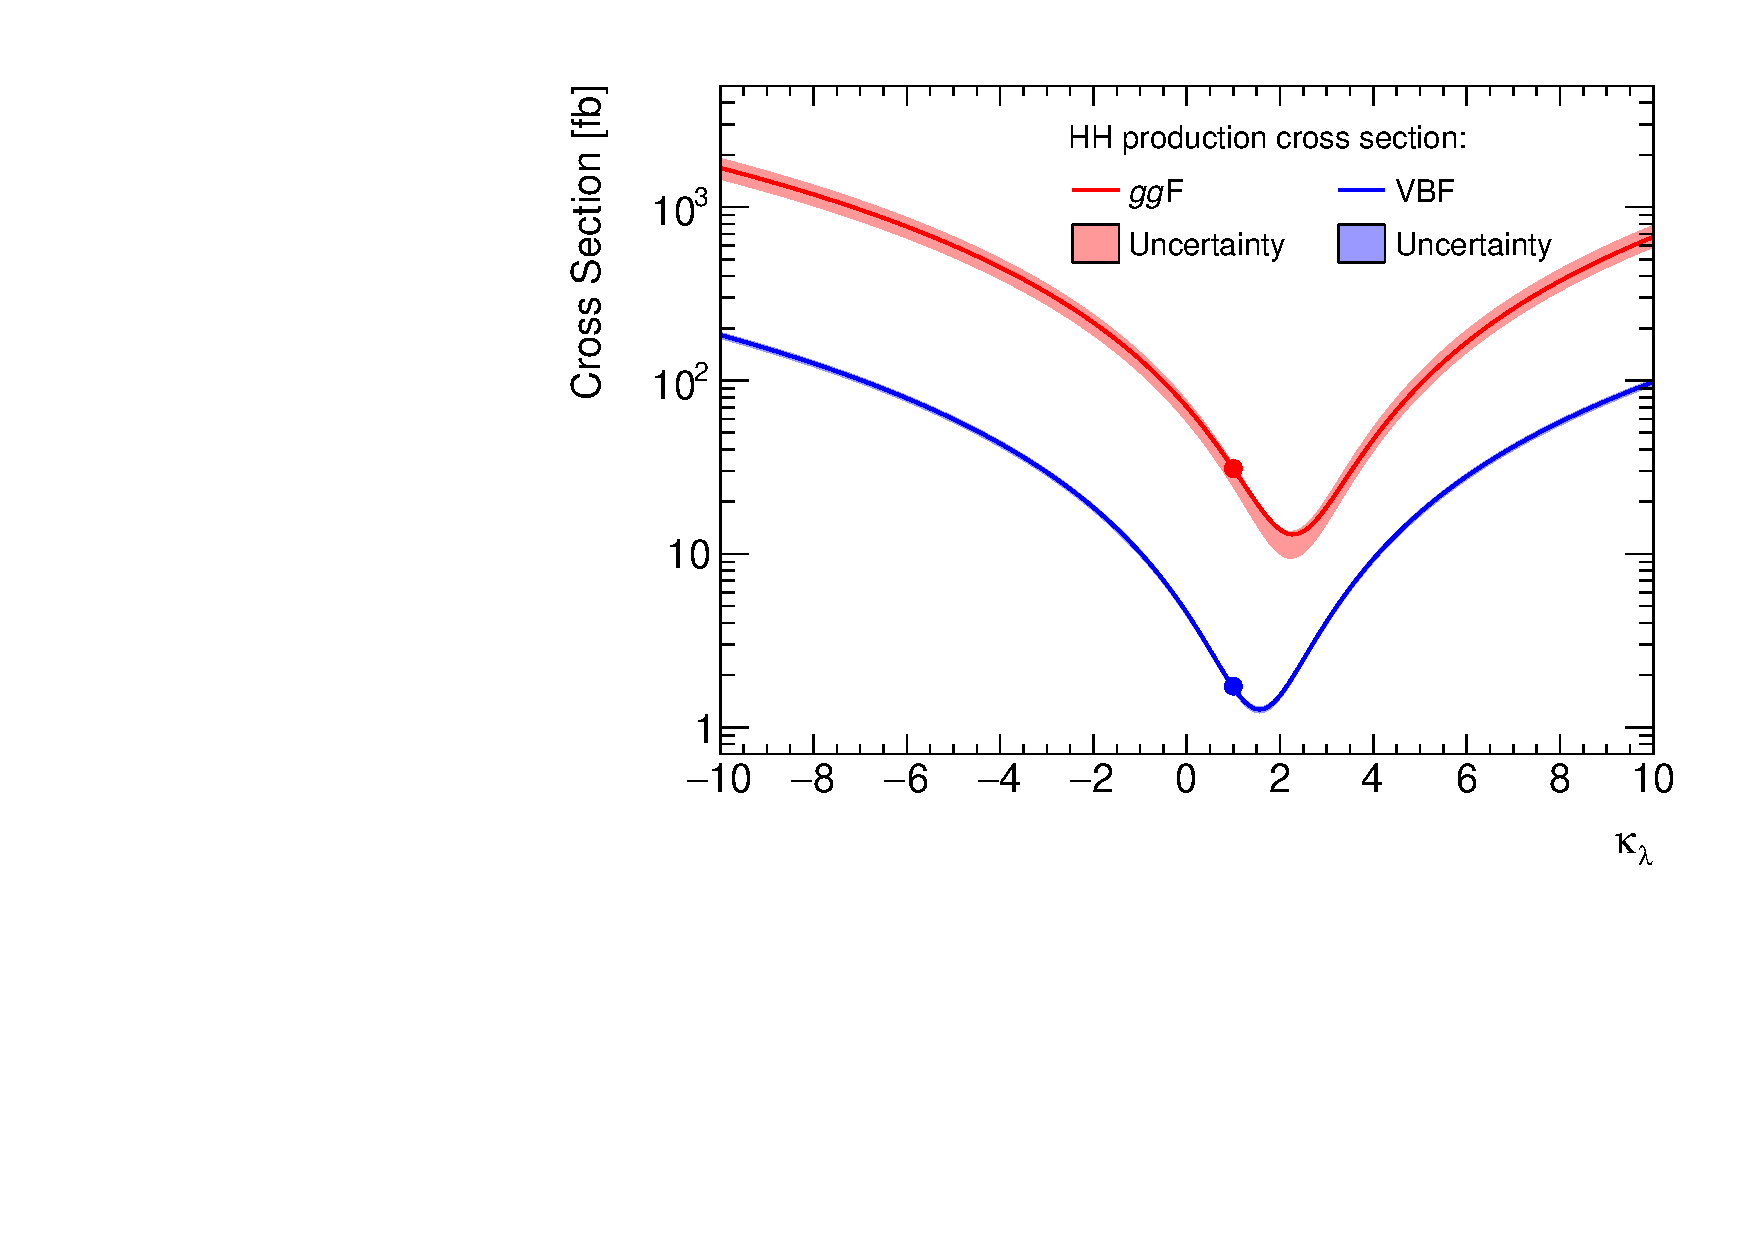
\includegraphics[width=0.55\textwidth]{self_coupling/hh_xsec}

  \caption{Higgs boson pair production cross section via the \ggF and VBF
    production modes as a function of \klambda. The production cross section for
    \ggF is given at $\text{NNLO}_{\text{NLO-i}}$ rescaled to
    $\text{NNLO}_{\text{FTapprox}}$~\cite{Grazzini:2018bsd} in the
    $\klambda = 1$ limit~\cite{Amoroso:2020lgh,Baglio:2020wgt,LHCHWGHH}. The
    production cross section via VBF is obtained from simulation with \MGNLO at
    LO after applying an $\text{N}^3\text{LO}$ $k$-factor derived for the SM
    case~\cite{Dreyer:2018qbw,LHCHWGHH}. The cross sections are parameterised as
    quadratic functions of \klambda. Theoretical uncertainties are shown as
    coloured bands.}%
  \label{fig:hh_xsec_incl}
\end{figure}

In addition to the change in total cross section, anomalous values of \klambda
alter the differential \HH production cross section in terms of the invariant
mass of the pair of Higgs bosons. This is shown in \Cref{fig:hh_xsec_mhh} for
the \ggF production mode and for five exemplary values of \klambda. The \mHH
spectra for different values of \klambda show large differences in their
\emph{hardness} as measured by the median of the \mHH distribution
in~\Cref{fig:hh_median_mhh}. For \klambda values just below or at the point of
maximum destructive interference between the box and triangle diagram, the \mHH
spectra are moderately hard and have a pronounced double peak structure. For
other values of \klambda, particularly for $\klambda \approx 3$, the cross
section at low \mHH is enhanced resulting in softer \mHH spectra.

\begin{figure}[htbp]
  \begin{subfigure}[t]{0.485\textwidth}
    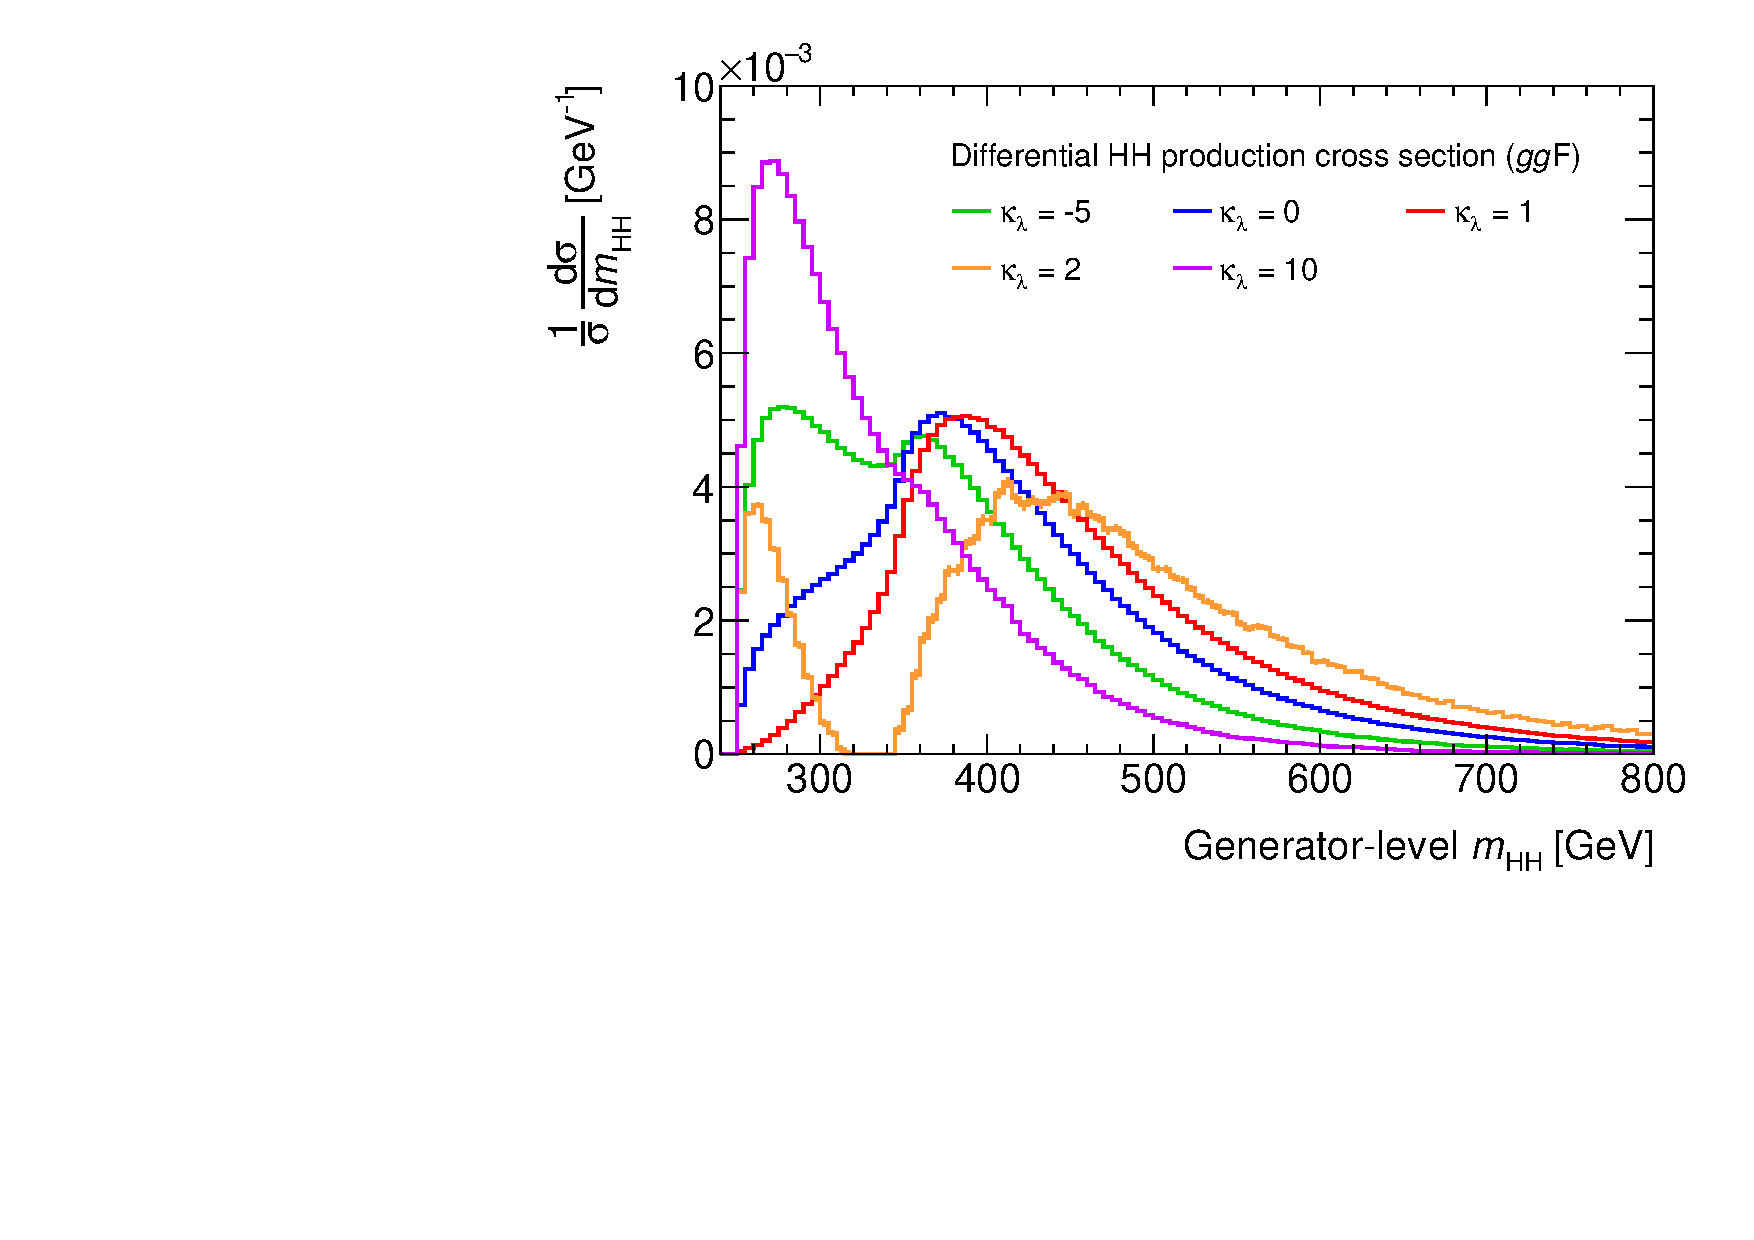
\includegraphics[width=\textwidth]{self_coupling/hh_mhh_vs_klam}
    \subcaption{%Differential \HH production cross section with respect
      %to \mHH for the \ggF production mode and selected values of
      %\klambda.
      % Differential cross sections are normalised by dividing by the
      % total cross section. Only statistical uncertainties from the
      % finite number of generated events are shown.
    }%
    \label{fig:hh_xsec_mhh}
  \end{subfigure}\hfill%
  \begin{subfigure}[t]{0.485\textwidth}
    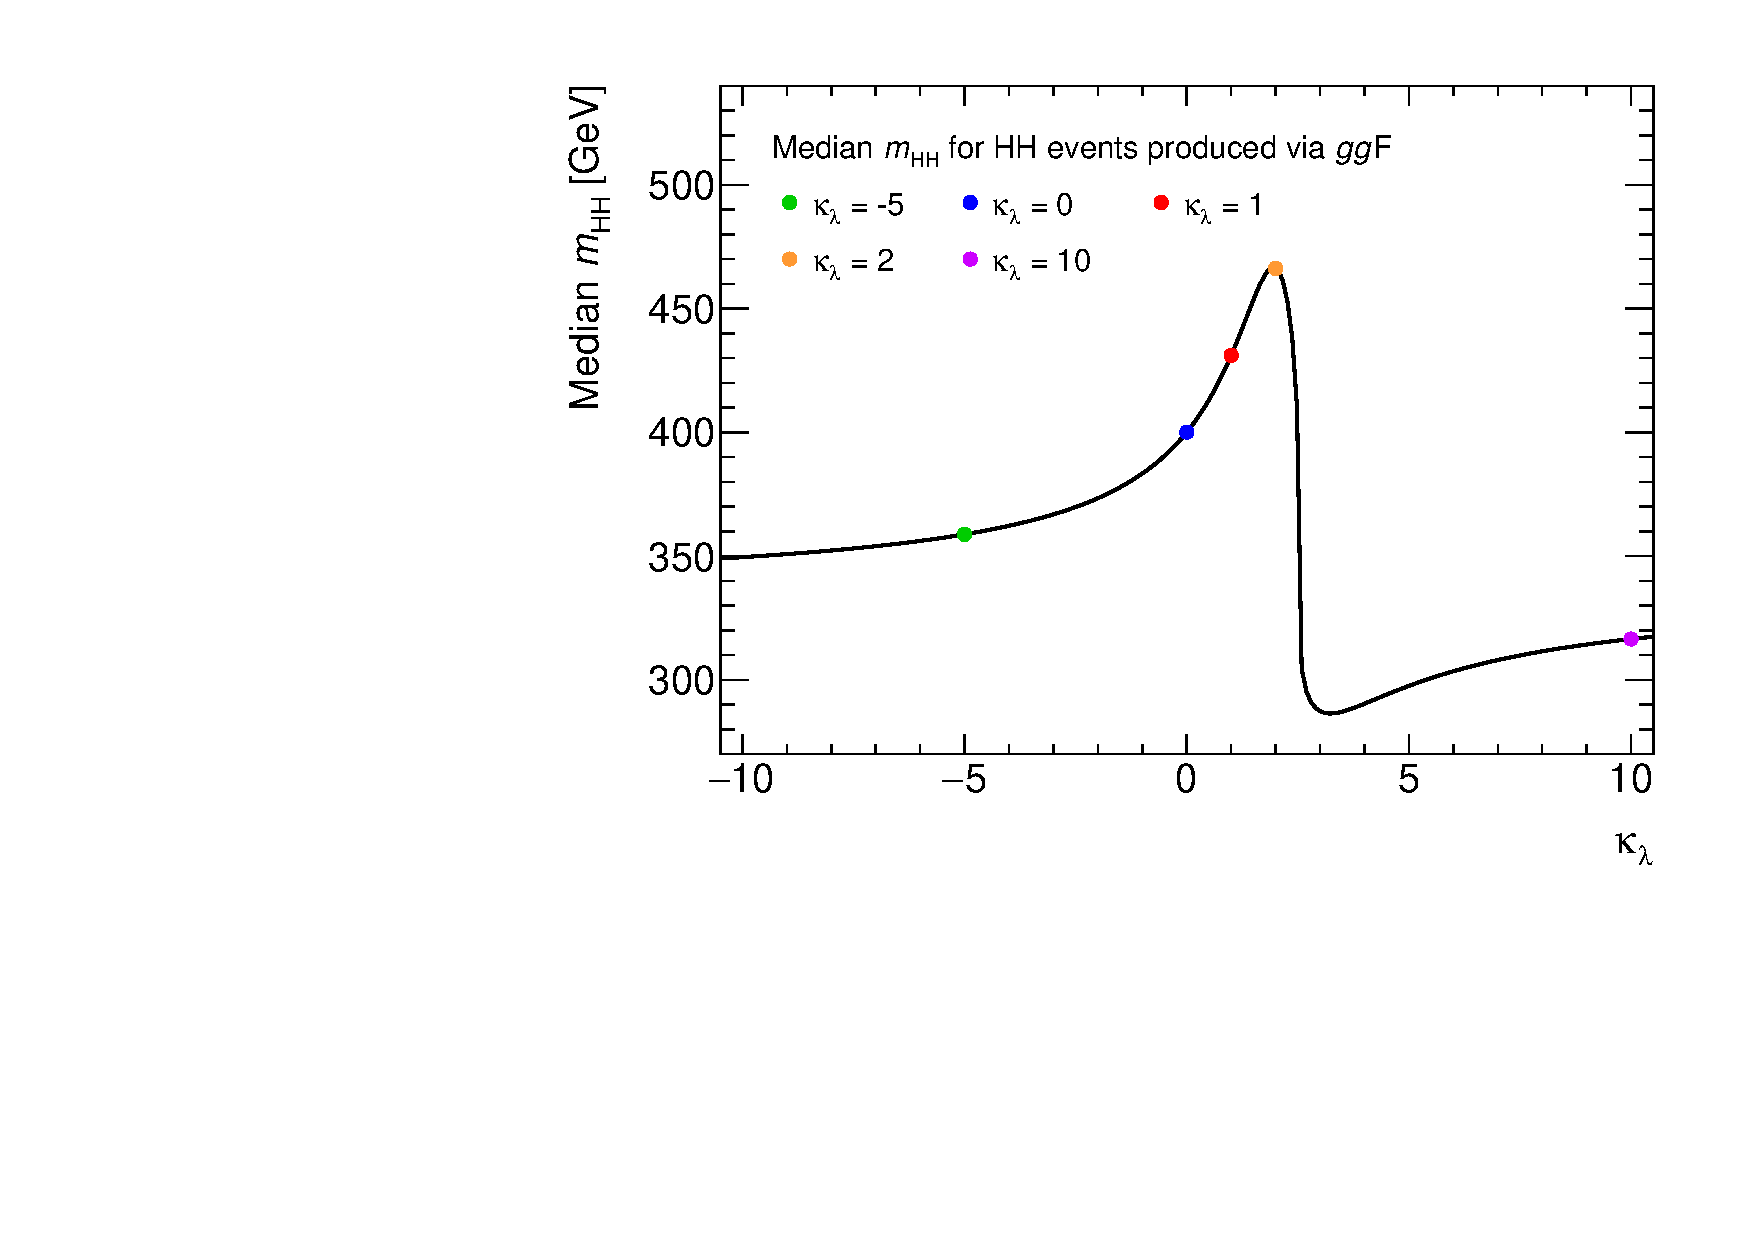
\includegraphics[width=\textwidth]{self_coupling/hh_median_mhh_vs_klam}
    \subcaption{%Median value of \mHH for Higgs boson pairs produced
      % via \ggF as a function of \klambda
    }%
    \label{fig:hh_median_mhh}
  \end{subfigure}

  \caption{Differential cross section of Higgs boson pair production
    with respect to \mHH for the \ggF production mode and selected
    values of \klambda (a) and the median value of \mHH as a function
    of \klambda (b). Both are given for \pp-collisions at
    $\sqrt{s} = \SI{13}{\TeV}$ and assuming $\mH =
    \SI{125.0}{\GeV}$. The cross sections are obtained from simulation
    with \POWHEGBOX[v2] at NLO including the top-quark mass
    dependence~\cite{Heinrich:2019bkc,Heinrich:2020ckp} for
    $\klambda = 0, 1, 10$. Differential cross sections for other
    values of \klambda are estimated using morphing techniques that
    are discussed in \Cref{sec:self_coupling_signals}.}
  \label{fig:xsec_median_mhh}
\end{figure}

The \klambda-dependency of $\mathrm{d}\sigma / \mathrm{d}\mHH$ is an
important factor affecting the sensitivity of searches to signals with
anomalous \klambda. This is due to experimental limitations in the
signal acceptance at low \mHH of most search channels due to
\pT-thresholds applied to objects at trigger-level. Particularly
searches targeting (visible) hadronic final states such as
$\bbbar\hadhad$ and \bbbb are affected. While these channels yield
stringent cross section limits for the SM case, scenarios where the
cross section at low \mHH is enhanced are less favourable due to the
high thresholds of $b$-jet and \tauhadvis triggers. In these cases,
the \bbyy channel, due to its use of di-photon triggers, yields larger
signal acceptance and the most stringent exclusion limits of a single
channel.


\section{Reinterpretation of the Search for SM \HH Production}%
\label{sec:reinterpretation}

The SM \HH search from \Cref{sec:dihiggs} is reinterpreted to set
upper limits on the cross section of non-resonant \HH production as a
function of an assumed valued of \klambda. %These upper limits allow,
%by comparison with the theoretical cross section predictions
%(cf.~\Cref{fig:hh_xsec_incl}), to exclude regions of \klambda that are
%incompatible with the observations made in the SM \HH search.
The reinterpretation adopts the statistical framework presented in
\Cref{sec:statistical_analysis} with few modifications. These
modifications are restricted to the signal model used in the
statistical interpretation. The background model and final
discriminants, including their binning, remain identical to those in
the SM \HH search.

The signal model used for the statistical interpretation is obtained by
replacing the SM \HH signal with signals from non-resonant \HH production with
arbitrary but fixed \klambda. Similar to the SM \HH search, the combination of
non-resonant \HH production via \ggF and VBF is considered as the signal
process. The signal is normalised using the total non-resonant \HH production
cross section via \ggF and VBF, \xsecggfvbf, which is allowed to vary freely and
is considered to be the POI.
% \footnote{The total cross section $\sigma_{\text{ggF+VBF}}$ is
% inclusive in the decay modes of the Higgs bosons. It is extrapolated
% from the measurement in the \bbtautau channel assuming Higgs boson
% branching ratios as predicted by the SM.}
The methods for obtaining signal templates in the signal regions are
described in \Cref{sec:self_coupling_signals}.

The adopted method of reinterpretation makes assumptions that are given in the
following: First, except for \klambda, all coupling strengths are assumed to be
at their SM values. Second, the single Higgs boson production cross sections and
branching ratios are fixed to their SM values and are thus assumed to be
independent of \klambda. This is generally not the case since variations of
\klambda affect both the production cross sections and branching ratios due to
electroweak corrections. These effects and their sensitivity to \klambda are
discussed in
Refs.~\cite{ATL-PHYS-PUB-2019-009,Degrassi:2016wml,Maltoni:2017ims}.  Since
backgrounds from single Higgs boson production are non-negligible in the SM \HH
search, it is instructive to gauge the crudeness of this approximation over the
allowed interval of $-5.0 < \klambda < 12.0$ from previous results of the ATLAS
collaboration~\cite{HDBS-2018-58}. In the considered \klambda interval, the
single Higgs boson production cross sections deviate from the SM prediction by
up to \SI{12}{\percent} (\SI{25}{\percent}) for the \ggF, VBF, and $VH$
($\ttbar H$) production modes~\cite{ATL-PHYS-PUB-2019-009}. The Higgs boson
branching ratios to fermions show small relative deviations of up to
\SI{3}{\percent} from the SM over the relevant \klambda
range~\cite{ATL-PHYS-PUB-2019-009}. For the purpose of this reinterpretation,
signal processes were generated assuming SM Higgs boson branching ratios for
consistency with the treatment of single Higgs boson backgrounds. The
assumptions about single Higgs boson production cross sections and branching
ratios were dropped in a follow-up analysis performed as part of
Ref.~\cite{HDBS-2022-03} by the ATLAS collaboration, which is briefly discussed
in the conclusion of this chapter.


\subsection{Signal Templates and Uncertainties}%
\label{sec:self_coupling_signals}

The distributions of the signal process in the three signal regions
and for various values of \klambda are required for the
reinterpretation.
% Templates of the contribution of a signal with anomalous values of
% \klambda in all three signal regions are required for the
% reinterpretation.
These are obtained using morphing and re-weighting techniques
developed by the ATLAS collaboration that are explained hereafter. An
ingredient for both methods are simulated event samples for different
assumed values of \klambda. The event simulation proceeds using the
same generator setup described in
\Cref{sec:data_and_simulation}. Events from non-resonant \HH
production are generated for $\klambda = 1, 10$ for the \ggF
production mode and $\klambda = 0, 1, 10, 20$ for the VBF production
mode. In addition, large samples of events from non-resonant \HH
production via \ggF are generated for $\klambda = 0, 1, 10, 20$
without simulation of the ATLAS detector. All event samples are
normalised using the cross sections previously shown in
\Cref{fig:hh_xsec_incl}.

Established morphing techniques~\cite{ATL-PHYS-PUB-2015-047} are used
to obtain signal templates for arbitrary \klambda by linearly
combining a set of basis templates with fixed \klambda. This approach
is motivated by considering the squared matrix element of non-resonant
\HH production for either the \ggF or VBF production mode at leading
order in \klambda. The squared matrix element can be written as
\begin{align*}
  |\mathcal{M}|^2 = \klambda^2 |\mathcal{A}|^2 + 2 \klambda \operatorname{Re}(\mathcal{A} \mathcal{B}^*) + |\mathcal{B}|^2 \,\text{,}
\end{align*}
where $\mathcal{A}$ is the (complex) amplitude of diagrams involving
the Higgs boson-self coupling after factoring out the value of the
anomalous self-coupling constant, and $\mathcal{B}$ the amplitude of
diagrams not involving any Higgs boson self-interactions. The
knowledge of $|\mathcal{M}|^2$ for three distinct values of \klambda
allows to calculate the squared matrix element for any value of
\klambda by solving for the squared amplitudes of $\mathcal{A}$ and
$\mathcal{B}$, and the interference term. The same considerations can
be applied to express the differential cross section for any \klambda
as a linear combination of predictions at $\klambda = a, b, c$
according to
% The same considerations apply to predictions of differential cross
% sections, such that the differential cross section at any \klambda
% can be obtained by linearly combining the predictions at
% $\klambda = a, b$ and $c$ according to
\begin{align*}
  \frac{\mathrm{d}\sigma}{\mathrm{d}\myvec{x}}(\klambda)
  = w_1(\klambda) \left. \frac{\mathrm{d}\sigma}{\mathrm{d}\myvec{x}} \right|_{\klambda = a}
  + w_2(\klambda) \left. \frac{\mathrm{d}\sigma}{\mathrm{d}\myvec{x}} \right|_{\klambda = b}
  + w_3(\klambda) \left. \frac{\mathrm{d}\sigma}{\mathrm{d}\myvec{x}} \right|_{\klambda = c} \,\text{,}
\end{align*}
where the coefficients $w_i(\klambda)$ are second degree polynomials
in \klambda and $\myvec{x}$ is an arbitrary variable characterising
the scattering process.\footnote{For non-resonant \HH production via
  \ggF, this method was documented by the ATLAS collaboration in
  Ref.~\cite{ATL-PHYS-PUB-2019-007}.}

For the \ggF production mode, this morphing technique is only used
indirectly. Differential distributions at generator-level are obtained
by linearly combining the $\klambda = 0, 1, 20$ event samples without
detector simulation. These distributions are used to derive a
re-weighting in bins of the generator-level \mHH that allows to
re-weight the $\klambda = 1$ event sample to any other value of
\klambda. The re-weighting is then applied to the $\klambda = 1$
sample with full detector simulation. This approach avoids having to
run the computationally expensive detector simulation for all event
samples required for the morphing technique. For the VBF production
mode, the morphing technique is used directly by performing linear
combinations of the $\klambda = 1, 2, 10$ event samples. In this case,
the re-weighting method is not used because the effects of \klambda
variations are not easily parameterised as a re-weighting in a single
variable. Event samples not used for morphing or re-weighting are used
for validation purposes.

Uncertainties on the modelling of the signal processes with anomalous
\klambda are derived according to \Cref{sec:modelling_uncertainties}.
Variations of the $H \to \tautau$ and $H \to \bbbar$ branching ratios,
the parton shower simulation, the renormalisation and factorisation
scales, and the PDFs and $\alphas$ are considered. Additionally, the
statistical uncertainties of the \klambda re-weighting factors are
accounted for.


\subsection{Signal Acceptance in the \bbtautau Channel}%
\label{sec:self_coupling_bbtt_limitations}

The strength of the $\bbbar\hadhad$ and $\bbbar\lephad$ SLT/LTT channels in
setting upper limits on the cross section of non-resonant \HH production can be
qualitatively understood by examining the signal acceptance of the channels as a
function of \klambda. The signal acceptance is shown in
\Cref{fig:acceptance_vs_klambda} for the signal region selections of the three
channels and their combination. It reaches a maximum at $\klambda \approx 2$,
which corresponds to the value of the self-coupling constant with the largest
median \mHH for signal events produced via \ggF
(cf.~\Cref{fig:xsec_median_mhh}). In addition, \Cref{fig:acceptance_vs_mhh}
depicts the signal acceptance in bins of the generator-level \mHH for the
dominant \ggF production mode, illustrating the limitations in selecting signal
events with low \mHH. While the \hadhad and \lephad SLT channels have similar
signal acceptances over a wide range of \mHH, the signal acceptance in the low
\mHH region is dominated by the \lephad SLT channel. The inclusion of the
\lephad LTT channel, which selects events with leptons below the lepton
\pT-threshold of the \lephad~SLT channel, is primarily intended to improve the
signal acceptance at low \mHH, which is where its relative contribution to the
total signal acceptance is largest.

\begin{figure}[htbp]
  \centering

  \begin{subfigure}[t]{0.485\textwidth}
    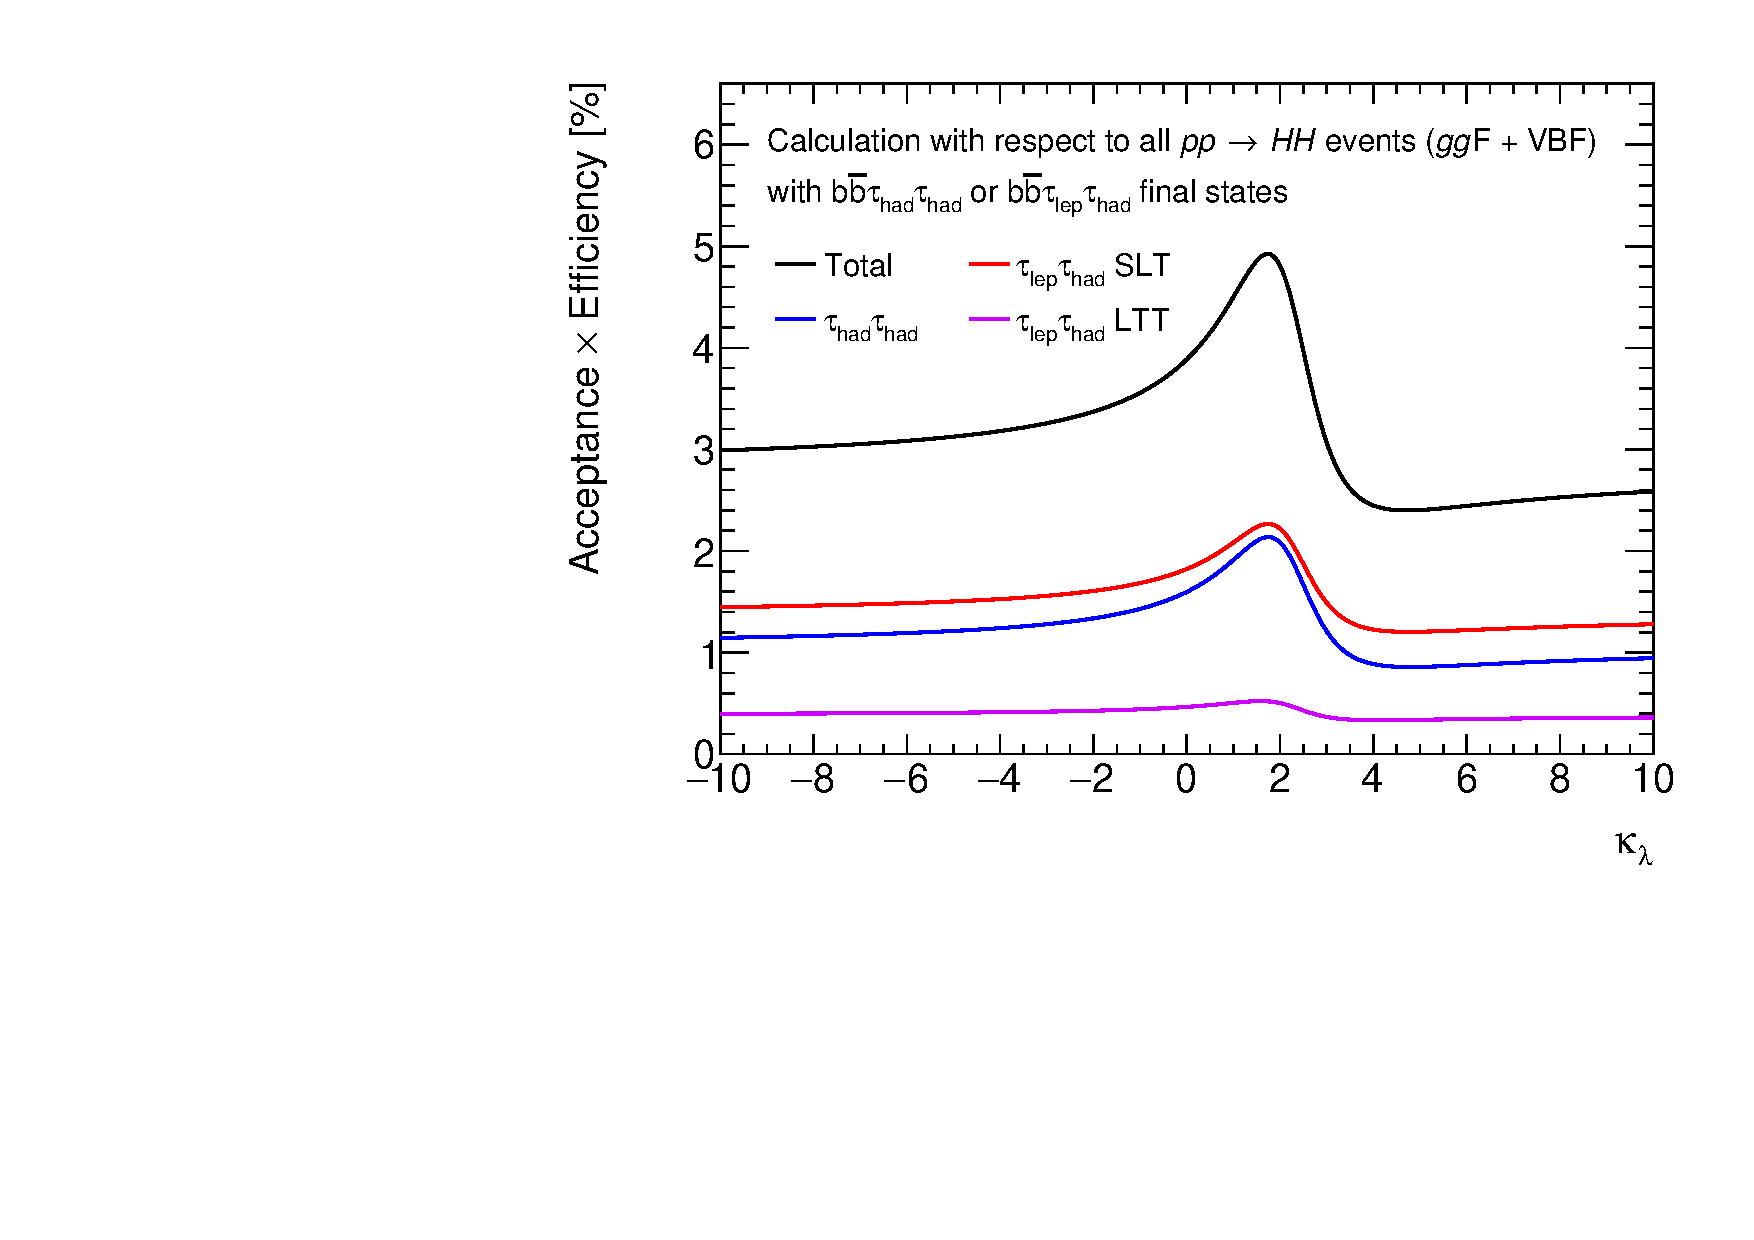
\includegraphics[width=\textwidth]{self_coupling/acc_vs_klam}
    \subcaption{Signal acceptance (\ggF + VBF) as a function of \klambda. The
      combination of all channels is shown in black.}%
    \label{fig:acceptance_vs_klambda}
  \end{subfigure}\hfill%
  \begin{subfigure}[t]{0.485\textwidth}
    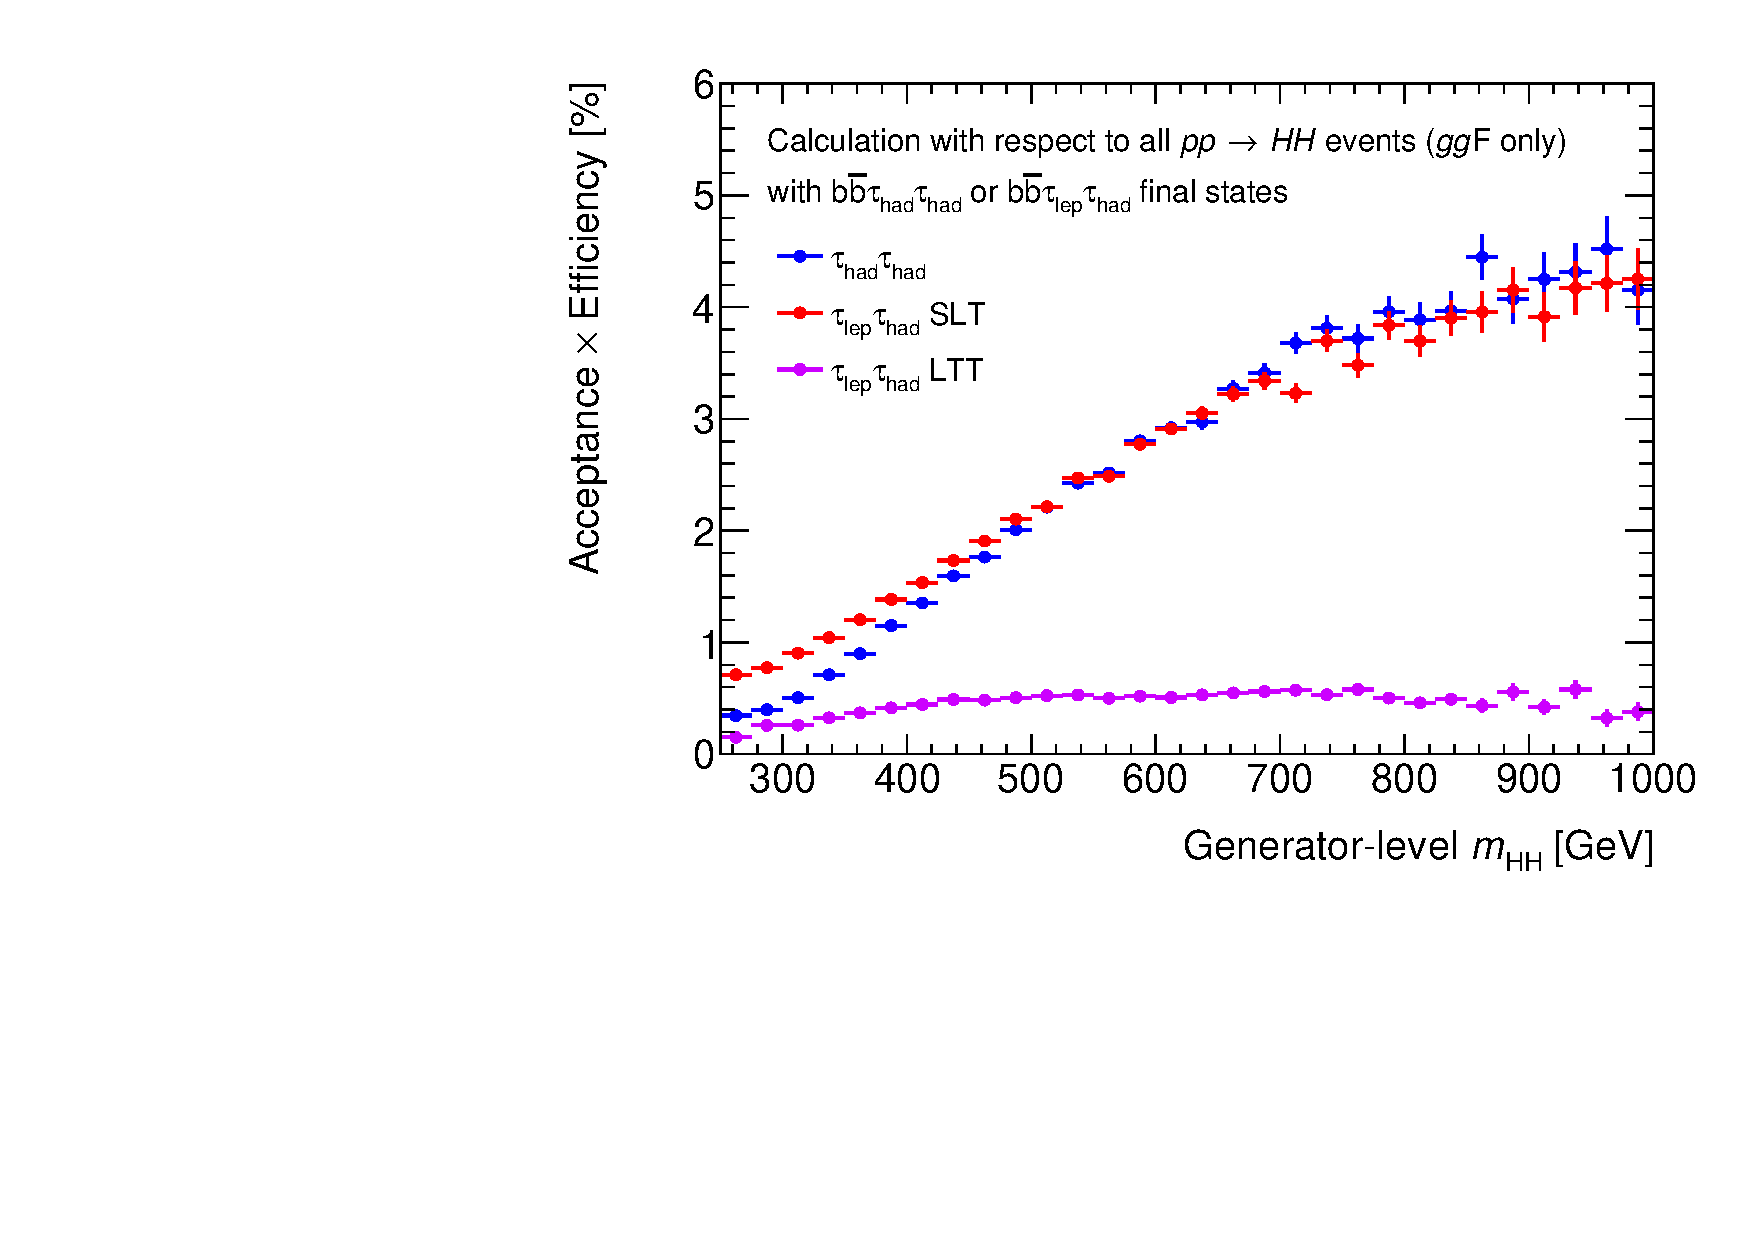
\includegraphics[width=\textwidth]{self_coupling/acc_vs_mhh}
    \subcaption{Signal acceptance (\ggF only) in bins of the generator-level
      \mHH.}%
    \label{fig:acceptance_vs_mhh}
  \end{subfigure}

  \caption{Acceptance of events from non-resonant \HH production in
    the \hadhad, \lephad~SLT, and \lephad~LTT channels. The signal
    acceptance is calculated as the fraction of events with
    $\bbbar\tauhad\tauhad$ or $\bbbar\taulep\tauhad$ final states
    passing the signal region selections of a given channel.}%
  \label{fig:acceptance_vs_klambda_vs_mhh}
\end{figure}

The signal acceptance is not the only factor in determining the sensitivity of
the reinterpretation. First, signals with enhanced cross sections at low \mHH
have a larger overlap with background processes.
% , thus leading to further reductions in signal sensitivity.
Second, the BDT used for signal extraction is trained to distinguish between
SM~\HH events and background events. Consequently, the signal-background
classification is biased towards events with large \mHH due to the moderately
hard \mHH spectrum of SM~\HH production. Both factors lead to further reductions
in sensitivity to signals with soft \mHH spectra.

% Signals with enhanced cross sections at low \mHH have larger overlap with
% background processes. This is a consequence of using multivariate
% discriminants trained to distinguish SM \HH events from backgrounds and the
% greater abundance of background events with low \mHH.


\section{Results}%
\label{sec:reinterpretation_results}

Upper limits are set on \xsecggfvbf at \SI{95}{\percent} CL by combining the
\hadhad, \lephad SLT, and \lephad LTT channels. The exclusion limits obtained by
the ATLAS collaboration are shown in~\Cref{fig:klambda_scan} as a function of
\klambda. They are compared to the prediction of the combined non-resonant \HH
production cross section via \ggF and VBF from theory, previously shown
in~\Cref{fig:hh_xsec_incl}. The most stringent limits are set for
$\klambda \approx 2$ which follows from signal acceptance considerations
discussed previously. The theory prediction of the non-resonant \HH production
cross section exceeds the observed upper limit outside of the interval of
\mbox{$\klambda \in [-2.4, 9.2]$}, thus excluding non-resonant \HH production
with \mbox{$\klambda \notin [-2.4, 9.2]$} based on the upper limits on the cross
sections.%\footnote{The allowed \klambda interval is not a confidence interval
  %with well-defined coverage properties. Such an interval would require a more
  %rigorous treatment that includes \klambda as a parameter in the statistical
  %model.}\fnsep
\footnote{The constraints on \klambda are largely driven by the \hadhad
  channel. An analysis of the \hadhad channel only yields observed (expected)
  \klambda intervals of $\klambda \in [ -2.5, 9.3
  ]$~($\klambda \in [ -2.3, 9.2 ]$), while the combination of the \lephad SLT
  and LTT channel yields $\klambda \in [ -3.8, 12.2
  ]$~($\klambda \in [ -3.8, 11.9 ]$)~\cite{Dimitriadi}.}

\begin{figure}[htbp]
  \centering

  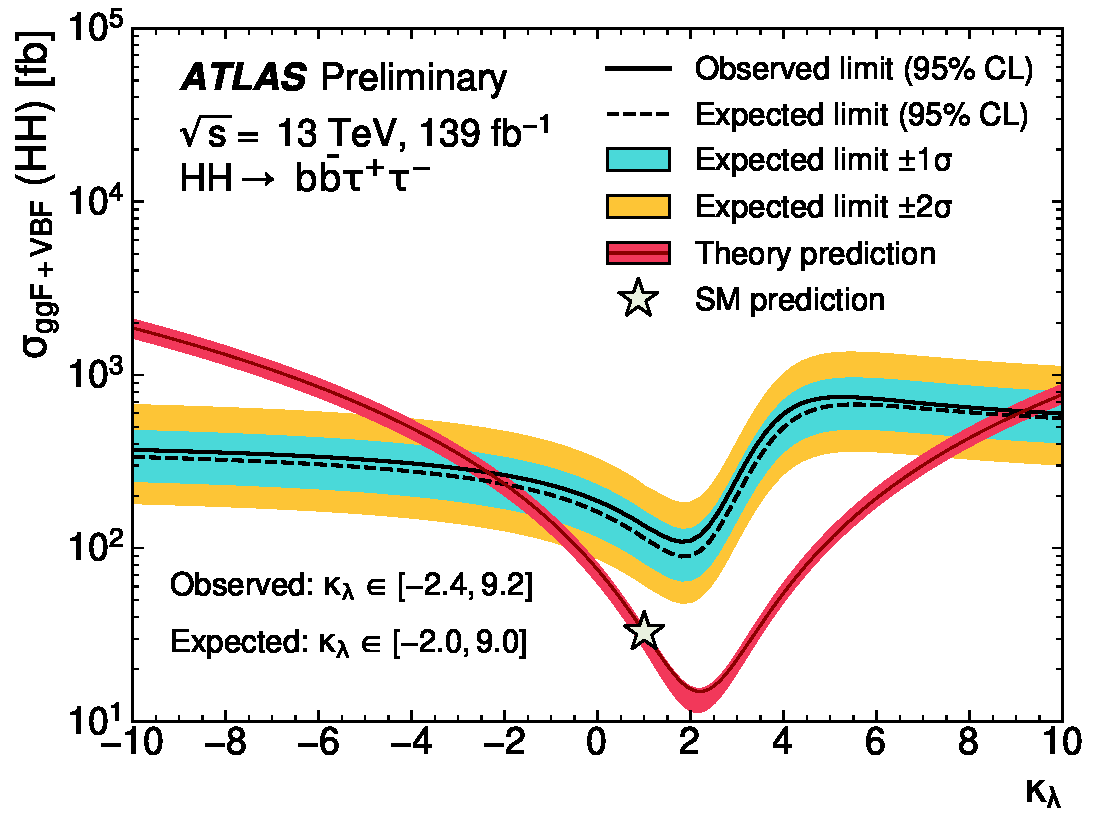
\includegraphics[width=0.58\textwidth]{self_coupling/klam_scan_result}

  \caption{Upper limits on the Higgs boson pair production cross
    section via \ggF and VBF, \xsecggfvbf, for the combination of the
    \hadhad, \lephad SLT, and \lephad LTT channels at
    \SI{95}{\percent} CL as a function of \klambda. The theory
    prediction previously described in \Cref{fig:hh_xsec_incl} is
    overlaid. The expected upper limits assume the absence of
    non-resonant \HH production~($\xsecggfvbf = 0$). The \klambda
    intervals defined by the intersection of the theory prediction
    with the observed/expected limits are given in the lower left of
    the figure. The figure is taken from
    Ref.~\cite{ATLAS-CONF-2021-052}.}%
  \label{fig:klambda_scan}
\end{figure}

This result represents a significant improvement over earlier searches by the
ATLAS collaboration using \SI{36}{\per\femto\barn} of \pp-collision data
collected at the start of Run~2 of the LHC. These searches yielded allowed
\klambda intervals of \mbox{$\klambda \in [-7.4, 15.7]$} and
\mbox{$\klambda \in [-5.0, 12.0]$} for the \bbtautau channel and the combination
of the \bbbb, \bbtautau, and \bbyy channels~\cite{HDBS-2018-58},
respectively. Due to the increased size of the \pp-collision dataset and the
analysis improvements in the \bbtautau channel, the reinterpretation presented
in this chapter puts more stringent constraints on \klambda than the earlier
combination of the most sensitive channels.

A comparison between the allowed \klambda intervals of searches in the \bbbb,
\bbtautau, and \bbyy channels performed at the end of Run~2 by the ATLAS
collaboration is given in \Cref{tab:allowed_klambda}. The results of searches in
the \bbtautau and \bbyy channels are complementary. While the \bbyy channel sets
more stringent upper bounds on the allowed \klambda interval due to its superior
acceptance of signal events with low \mHH, the \bbtautau channel provides a
lower bound that is competitive with the result of the \bbyy channel. The \bbbb
channel is the third most sensitive channel due to its limited signal acceptance
and large multi-jet backgrounds, however, these disadvantages are partially
compensated by the large $H \to \bbbar$ branching ratio. Lastly, the
corresponding results of the CMS collaboration are summarised in
\Cref{tab:cms_klambda} showing similar findings as those of the ATLAS
collaboration.

\begin{table}[htbp]
  \caption{Allowed \klambda intervals from searches for non-resonant \HH
    production in \bbbb, \bbtautau, and \bbyy channels by the ATLAS and CMS
    collaborations using \pp-collision datasets collected during Run~2 of the
    LHC. The expected \klambda intervals are derived from the expected upper
    limits on \xsecggfvbf under the background-only ($\xsecggfvbf = 0$)
    hypothesis.}

  \begin{subfigure}[t]{\textwidth}
    \centering

    \subcaption{Results of the ATLAS collaboration with an integrated luminosity
      of up to \SI{139}{\per\femto\barn}. $\dagger$: The integrated luminosity
      of the search in the \bbbb channel amounts to \SI{126}{\per\femto\barn}.}%
    \label{tab:allowed_klambda}

    \begin{tabular}{lccc}
      \toprule
      \textbf{ATLAS} & \multicolumn{3}{c}{Allowed \klambda interval} \\
      \cmidrule{2-4}
      Search channel & Observed & Expected & Reference  \\
      \midrule
      $\bbbb^\dagger$     & $[-3.9, 11.1]$           & $[-4.6, 10.8]$           & \cite{ATLAS-CONF-2022-035} \\
      \bbtautau & $[-2.4, \phantom{0}9.2]$ & $[-2.0, \phantom{0}9.0]$ & \cite{ATLAS-CONF-2021-052} \\
      \bbyy     & $[-1.5, \phantom{0}6.7]$ & $[-2.4, \phantom{0}7.7]$ & \cite{HDBS-2018-34} \\
      \bottomrule
    \end{tabular}
  \end{subfigure}

  \vspace{1em}

  \begin{subfigure}[t]{\textwidth}
    \centering

    \subcaption{Results of the CMS collaboration with an integrated luminosity
      of \SI{138}{\per\femto\barn}. $\ddag$: The search in the \bbyy channel
      accounts for the change in single Higgs boson production cross section and
      branching ratio with \klambda.}%
    \label{tab:cms_klambda}

    \begin{tabular}{lccc}
      \toprule
      \textbf{CMS} & \multicolumn{3}{c}{Allowed \klambda interval} \\
      \cmidrule{2-4}
      Search channel & Observed & Expected & Reference  \\
      \midrule
      \bbbb     & $[-2.3, \phantom{0}9.4]$ & $[-5.0, 12.0]$            & \cite{CMS-HIG-20-005} \\
      \bbtautau & $[-1.7, \phantom{0}8.7]$ & $[-2.9, \phantom{0}9.8]$  & \cite{CMS-HIG-20-010} \\
      $\bbyy^\ddag$     & $[-3.3, \phantom{0}8.5]$ & $[-2.5, \phantom{0}8.2]$  & \cite{CMS-HIG-19-018} \\
      \bottomrule
    \end{tabular}
  \end{subfigure}
\end{table}


\section{Conclusion and Outlook}%
\label{sec:reinterpretation_conclusion}

An interpretation of the search for non-resonant \HH production in the \bbtautau
channel in terms of anomalous Higgs boson self-coupling strengths is
presented. Upper limits at \SI{95}{\percent} CL are set on the total cross
section of Higgs boson pair production via \ggF and VBF as a function of the
self-coupling constant. An allowed range of
\begin{align*}
  &-2.4 \leq \klambda \leq 9.2 \text{ (observed)}
  && -2.0 \leq \klambda \leq 9.0 \text{ (expected for $\xsecggfvbf = 0$)}
\end{align*}
is obtained by comparing the cross section exclusion limits at
\SI{95}{\percent}~CL with cross section predictions from theory. The results are
based on the assumption that other coupling constants are at their SM values. In
addition, changes in single Higgs boson production cross sections and Higgs
boson branching ratios due variations of \klambda are neglected.

A follow-up analysis is performed by the ATLAS collaboration in
Ref.~\cite{HDBS-2022-03} that combines the results of the \bbbb, \bbtautau, and
\bbyy channels to perform a direct measurement of \klambda.  Similar to the
analysis presented in this chapter, the follow-up analysis includes the results
of the SM~\HH search from \Cref{sec:dihiggs} as part of the
reinterpretation. The main differences with respect to this chapter are as
follows: First, the statistical model uses \klambda as the POI, allowing to
estimate \klambda confidence intervals using likelihood ratio tests. Second, the
\klambda-dependencies of single Higgs boson production cross sections and Higgs
boson branching ratios are accounted for.
% In contrast to the method presented in this chapter, the statistical model is
% constructed using \klambda as a parameter of interest, allowing to obtain
% confidence intervals using likelihood-ratio tests. Moreover, the
% \klambda-dependency of single Higgs boson production and the Higgs boson decay
% was accounted for.
The follow-up analysis estimates \klambda confidence intervals at
\SI{95}{\percent}~CL for the combination of the \bbbb, \bbtautau, and \bbyy
channels to be $\klambda \in [-0.6, 6.6]$ for the observed data and
$\klambda \in [-2.1, 7.8]$ for the expectation under the $\klambda = 1$
hypothesis~\cite{HDBS-2022-03}. When considering only the search in the
\bbtautau channel, the \klambda confidence intervals are
\begin{align*}
  &-2.7 \leq \klambda \leq 9.5 \text{ (observed)}
  &&-3.1 \leq \klambda \leq 10.2 \text{ (expected for $\klambda = 1$)}
\end{align*}
at \SI{95}{\percent}~CL~\cite{hepdata.h_hh_comb}.\todo{Update HEPData link once
  available.}
% H+HH comb results for bbtautau only (from HEPData)
% https://atlas-glance.cern.ch/atlas/analysis/papers/details.php?id=14590
% Expected: [-3.1, 10.2]
% Observed: [-2.7, 9.5]
The observed \klambda confidence intervals show decent agreement with the result
obtained in this chapter that neglected \klambda-dependent electroweak
corrections. The expected \klambda intervals are derived under different
assumptions, therefore, larger differences are expected.

Probing the nature of the Higgs boson self-coupling is an important physics goal
of the HL-LHC. Prospects of the sensitivity to the self-coupling constant with
\SI{3000}{\per\femto\barn} \pp-collision data at $\sqrt{s} = \SI{14}{\GeV}$ were
derived in Ref.~\cite{ATL-PHYS-PUB-2021-044} by projecting the results of the SM
\HH search in the \bbtautau channel. This extrapolation yields an expected
confidence interval of $\klambda \in [-0.3, 7.4]$ at \SI{95}{\percent} CL
assuming the $\klambda = 1$ hypothesis~\cite{ATL-PHYS-PUB-2021-044}. By
combining with projections in the \bbyy channel~\cite{ATL-PHYS-PUB-2022-001},
first exclusion of the $\klambda = 0$ hypothesis at \SI{95}{\percent} CL could
be achieved using the dataset collected at the
HL-LHC~\cite{ATL-PHYS-PUB-2022-005}. This would represent a first milestone in
experimentally supporting the Higgs boson self-interaction predicted by the SM,
showing that a model without Higgs boson self-coupling would be disfavoured.

% Prospects for HL-LHC \SI{95}{\percent} CL\\
% Baseline (bbtautau): [-0.3, 7.4]\\
% Baseline (bbyy): [-0.2, 4.6]\\
% Baseline (bbyy + bbtautau): [0.0, 2.7]

% The total Higgs boson pair production cross section with anomalous
% couplings. Following recommendations by the LHC Higgs Working
% Group~\cite{LHCHWGHH}:
% \begin{description}

% \item[\ggF production mode] The cross sections of \HH production with
%   anomalous self-couplings were calculated in
%   Ref.~\cite{Amoroso:2020lgh} at $\text{NNLO}_{\text{NLO-i}}$
%   (NLO-improved). This prediction is obtained from combining the
%   result with the full top-quark mass dependence at
%   NLO~\cite{Buchalla:2018yce}


%   with NNLO corrections in the $m_{t} \to \infty$
%   limit~\cite{deFlorian:2017qfk}.

%   Additionally, the prediction is rescaled such that it coincides with
%   the SM \HH cross section at $\text{NNLO}_{\text{FTapprox}}$ at
%   $\klambda = 1$.

%   The total \HH production cross section via \ggF was found to depend
%   quadratically on \klambda and is thus parameterised
%   accordingly~\cite{LHCHWGHH}.

% \item[VBF production mode]

% \end{description}

% \todo[inline]{Read YR about Higgs cross section predictions:
%   \url{https://cds.cern.ch/record/2227475/files/CERN-2017-002-M.pdf}}


%%% Local Variables:
%%% mode: latex
%%% TeX-master: "../../phd_thesis"
%%% End:
